\vspace{1em}
\textbf{3.4. Сводная информация о рассмотренных методах.} 
\vspace{0.5em}

\begin{table}[h!]\hspace{-1em}
\begin{tabular}{|l|l|l|l|}
    \hline
    Метод             & Количество операций & Объём пересылок & Необходимая память \\
    \hline
    Рунге-Кутты       & $O(N^2)$            & $16Np$          & $6 N^2$ \\
    \hline
    С БПФ при $N=2^k$ & $O(N^2\log(N))$     & $O(N\log(N))p$    & $N^2 \text{ или } 2 N^2$ \\
    \hline
    С неявной схемой  & $O(N^2)$            & $4Np$           & $2 N^2$ \\
    \hline
\end{tabular}
\\[1ex]
\caption{Оценки количества вычислительных операций, сетевых обращений и потребляемой памяти рассматриваемыми методами.}
\label{tab:MethodsSummary}
\end{table}

\newpage
%\vspace{1em}
\noindent \textbf{4. Результаты.}
\vspace{0.5em}

Ниже представлены результаты замеров времени работы алгоритма с использованием преобразования Фурье при различных комбинациях параметров,
выбранных для анализа их влияния на время работы программы.
Замеры времени осуществлялись на кластере СКИФ МГУ <<Чебышёв>> 10 раз в разное время суток и усреднялись.

%%%%%%%%%%%%%%%%%%%%%%%%%%%%%%%%%%%%%%%%

    \begin{figure}[h!]
        \begin{center}
            \begin{minipage}{0.45\linewidth}
                \center{Флаг FFTW\_ESTIMATE:\\ \includegraphics[width=0.95\linewidth]{\graphsdir/Skif/FFTW_compare_N512_nomeasure_2k}}
                \caption{Время работы Фурье-алгоритма в зависимости от количества процессов. Размер матрицы $512 \times 512$. }
                \label{gr:Fourier512Nomeasure}
            \end{minipage}
            \hfill
            \begin{minipage}{0.45\linewidth}
                \center{Флаг FFTW\_MEASURE:\\ \includegraphics[width=0.95\linewidth]{\graphsdir/Skif/FFTW_compare_N512_measure_2k}}
                \caption{Время работы Фурье-алгоритма в зависимости от количества процессов. Размер матрицы $512 \times 512$.}
                \label{gr:Fourier512Measure}
            \end{minipage}
        \end{center}
    \end{figure}

    \begin{figure}[h!]
        \begin{center}
            \begin{minipage}{0.45\linewidth}
                \center{\includegraphics[width=0.95\linewidth]{\graphsdir/Skif/FFTW_compare_N2048_nomeasure_2k}}
                \caption{Время работы Фурье-алгоритма в зависимости от количества процессов. Размер матрицы $2048 \times 2048$.}
                \label{gr:Fourier2048Nomeasure}
            \end{minipage}
            \hfill
            \begin{minipage}{0.45\linewidth}
                \center{\includegraphics[width=0.95\linewidth]{\graphsdir/Skif/FFTW_compare_N2048_measure_2k}}
                \caption{Время работы Фурье-алгоритма в зависимости от количества процессов. Размер матрицы $2048 \times 2048$.}
                \label{gr:Fourier2048Measure}
            \end{minipage}
        \end{center}
    \end{figure}

    \begin{figure}[h!]
        \begin{center}
            \begin{minipage}{0.45\linewidth}
                \center{\includegraphics[width=0.95\linewidth]{\graphsdir/Skif/FFTW_compare_N8192_nomeasure_2k}}
                \caption{Время работы Фурье-алгоритма в зависимости от количества процессов. Размер матрицы $8192 \times 8192$.}
                \label{gr:Fourier8192Nomeasure}
            \end{minipage}
            \hfill
            \begin{minipage}{0.45\linewidth}
                \center{\includegraphics[width=0.95\linewidth]{\graphsdir/Skif/FFTW_compare_N8192_measure_2k}}
                \caption{Время работы Фурье-алгоритма в зависимости от количества процессов. Размер матрицы $8192 \times 8192$.}
                \label{gr:Fourier8192Measure}
            \end{minipage}
        \end{center}
    \end{figure}

    \newpage

%%%%%%%%%%%%%%%%%%%%%%%%%%%%%%%%%%%%%%%%

    \begin{figure}[h!]
        \begin{center}
            \begin{minipage}{0.48\linewidth}
                \center{\includegraphics[width=0.95\linewidth]{\graphsdir/Skif/FFTW_time_nosave_all}} \\
                \caption{Время работы Фурье-алгоритма в зависимости от количества процессов. Сохранение данных в файл не производилось.}
                \label{gr:TimeFourierNosave}
            \end{minipage}
            \hfill
            \begin{minipage}{0.48\linewidth}
                \center{\includegraphics[width=0.95\linewidth]{\graphsdir/Skif/FFTW_time_withsave_all}} \\
                \caption{Время работы Фурье-алгоритма в зависимости от количества процессов. Сохранение данных в файл производилось на каждом десятом шаге.}
                \label{gr:TimeFourierSave}
            \end{minipage}
        \end{center}
    \end{figure}

    \begin{figure}[h!]
        \begin{center}
            \begin{minipage}{0.48\linewidth}
                \center{\includegraphics[width=0.95\linewidth]{\graphsdir/Skif/FFTW_acceleration_nosave_2k}} \\
                \caption{Ускорение Фурье-алгоритма в зависимости от количества процессов. Сохранение данных в файл не производилось.}
                \label{gr:SpeedupFourierNosave}
            \end{minipage}
            \hfill
            \begin{minipage}{0.48\linewidth}
                \center{\includegraphics[width=0.95\linewidth]{\graphsdir/Skif/FFTW_acceleration_withsave_2k}} \\
                \caption{Ускорение Фурье-алгоритма в зависимости от количества процессов. Сохранение данных в файл производилось на каждом десятом шаге.}
                \label{gr:SpeedupFourierSave}
            \end{minipage}
        \end{center}
    \end{figure}

    \begin{figure}[h!]
        \begin{center}
            \begin{minipage}{0.48\linewidth}
                \center{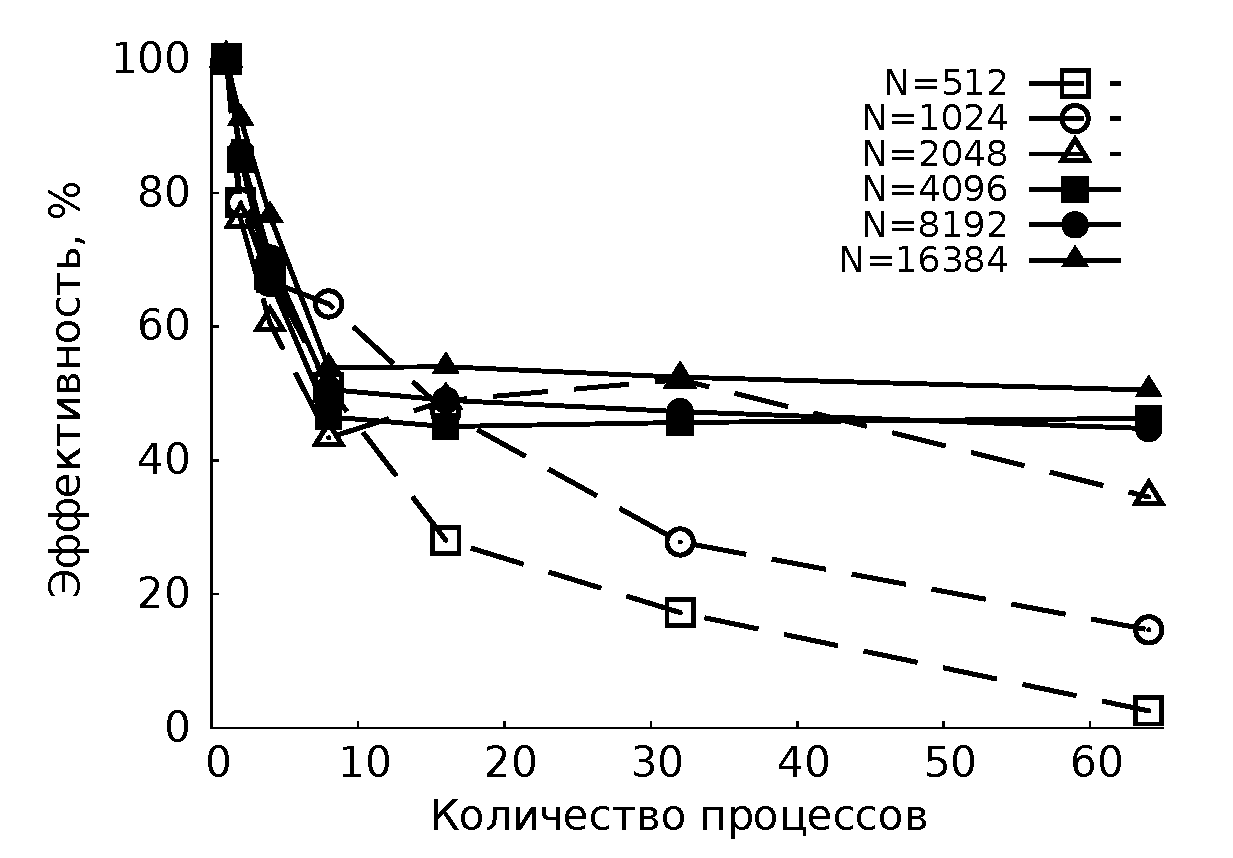
\includegraphics[width=0.95\linewidth]{\graphsdir/Skif/FFTW_efficiency_nosave_2k}} \\
                \caption{Эффективность Фурье-алгоритма в зависимости от количества процессов. Сохранение данных в файл не производилось.}
                \label{gr:EfficiencyFourierNosave}
            \end{minipage}
            \hfill
            \begin{minipage}{0.48\linewidth}
                \center{\includegraphics[width=0.95\linewidth]{\graphsdir/Skif/FFTW_efficiency_withsave_2k}} \\
                \caption{Эффективность Фурье-алгоритма в зависимости от количества процессов. Сохранение данных в файл производилось на каждом десятом шаге.}
                \label{gr:EfficiencyFourierSave}
            \end{minipage}
        \end{center}
    \end{figure}

    \newpage

%%%%%%%%%%%%%%%%%%%%%%%%%%%%%%%%%%%%%%%%

    \begin{figure}[h!]
        \begin{center}
            \begin{minipage}{0.45\linewidth}
                \center{
                    \includegraphics[width=0.95\linewidth]{\graphsdir/Skif/Sweep_time_nosave_all}
                }
                \caption{Время работы алгоритма с неявной схемой в зависимости от количества процессов. Сохранение данных в файл не производилось.}
                \label{gr:SweepTimeSkifNosave}
            \end{minipage}
            \hfill
            \begin{minipage}{0.45\linewidth}
                \center{
                    \includegraphics[width=0.95\linewidth]{\graphsdir/Skif/Sweep_time_withsave_all}
                }
                \caption{Время работы алгоритма с неявной схемой в зависимости от количества процессов. Сохранение данных в файл производилось на каждом десятом шаге.}
                \label{gr:SweepTimeSkifSave}
            \end{minipage}
        \end{center}
    \end{figure}

    \begin{figure}[h!]
        \begin{center}
            \begin{minipage}{0.45\linewidth}
                \center{
                    \includegraphics[width=0.95\linewidth]{\graphsdir/Skif/Sweep_acceleration_nosave_all}
                }
                \caption{Ускорение алгоритма с неявной схемой в зависимости от количества процессов. Сохранение данных в файл не производилось.}
                \label{gr:SweepSpeedupSkifNosave}
            \end{minipage}
            \hfill
            \begin{minipage}{0.45\linewidth}
                \center{
                    \includegraphics[width=0.95\linewidth]{\graphsdir/Skif/Sweep_acceleration_withsave_all}
                }
                \caption{Ускорение алгоритма с неявной схемой в зависимости от количества процессов. Сохранение данных в файл производилось на каждом десятом шаге.}
                \label{gr:SweepSpeedupSkifSave}
            \end{minipage}
        \end{center}
    \end{figure}

    \begin{figure}[h!]
        \begin{center}
            \begin{minipage}{0.45\linewidth}
                \center{
                    \includegraphics[width=0.95\linewidth]{\graphsdir/Skif/Sweep_efficiency_nosave_all}
                }
                \caption{Эффективность алгоритма с неявной схемой в зависимости от количества процессов. Сохранение данных в файл не производилось.}
                \label{gr:SweepEfficiencySkifNosave}
            \end{minipage}
            \hfill
            \begin{minipage}{0.45\linewidth}
                \center{
                    \includegraphics[width=0.95\linewidth]{\graphsdir/Skif/Sweep_efficiency_withsave_all}
                }
                \caption{Эффективность алгоритма с неявной схемой в зависимости от количества процессов. Сохранение данных в файл производилось на каждом десятом шаге.}
                \label{gr:SweepEfficiencySkifSave}
            \end{minipage}
        \end{center}
    \end{figure}

    \newpage

%%%%%%%%%%%%%%%%%%%%%%%%%%%%%%%%%%%%%%%%

    \begin{figure}[h!]
        \begin{center}
            \begin{minipage}{0.45\linewidth}
                \center{
                    \includegraphics[width=0.95\linewidth]{\graphsdir/Bluegene/Sweep_time_nosave_all}
                }
                \caption{Время работы алгоритма с неявной схемой на кластере IBM BlueGene/P. Сохранение данных в файл не производилось.}
                \label{gr:SweepTimeBluegeneNosave}
            \end{minipage}
            \hfill
            \begin{minipage}{0.45\linewidth}
                \center{
                    \includegraphics[width=0.95\linewidth]{\graphsdir/Bluegene/Sweep_time_withsave_all}
                }
                \caption{Время работы алгоритма с неявной схемой на кластере IBM BlueGene/P. Сохранение данных в файл производилось на каждом десятом шаге.}
                \label{gr:SweepTimeBluegeneSave}
            \end{minipage}
        \end{center}
    \end{figure}

    \begin{figure}[h!]
        \begin{center}
            \begin{minipage}{0.45\linewidth}
                \center{
                    \includegraphics[width=0.95\linewidth]{\graphsdir/Bluegene/Sweep_acceleration_nosave_all}
                }
                \caption{Ускорение параллельного алгоритма с неявной схемой на кластере IBM BlueGene/P. \mbox{Сохранение} данных в файл не производилось.}
                \label{gr:SweepSpeedupBluegeneNosave}
            \end{minipage}
            \hfill
            \begin{minipage}{0.45\linewidth}
                \center{
                    \includegraphics[width=0.95\linewidth]{\graphsdir/Bluegene/Sweep_acceleration_withsave_all}
                }
                \caption{Ускорение параллельного алгоритма с неявной схемой на кластере IBM BlueGene/P. \mbox{Сохранение} данных в файл производилось на каждом десятом шаге.}
                \label{gr:SweepSpeedupBluegeneSave}
            \end{minipage}
        \end{center}
    \end{figure}

    \begin{figure}[h!]
        \begin{center}
            \begin{minipage}{0.45\linewidth}
                \center{
                    \includegraphics[width=0.95\linewidth]{\graphsdir/Bluegene/Sweep_efficiency_nosave_all}
                }
                \caption{Эффективность параллельного алгоритма с неявной схемой на кластере IBM BlueGene/P. \mbox{Сохранение} данных в файл не производилось.}
                \label{gr:SweepEfficiencyBluegeneNosave}
            \end{minipage}
            \hfill
            \begin{minipage}{0.45\linewidth}
                \center{
                    \includegraphics[width=0.95\linewidth]{\graphsdir/Bluegene/Sweep_efficiency_withsave_all}
                }
                \caption{Эффективность параллельного алгоритма с неявной схемой на кластере IBM BlueGene/P. \mbox{Сохранение} данных в файл производилось на каждом десятом шаге.}
                \label{gr:SweepEfficiencyBluegeneSave}
            \end{minipage}
        \end{center}
    \end{figure}

    \newpage

%%%%%%%%%%%%%%%%%%%%%%%%%%%%%%%%%%%%%%%%

Из представленных на рис. \ref{gr:Fourier512Nomeasure}, \ref{gr:Fourier512Measure} графиков видно, что использование более 8 процессоров является неэффективным для матрицы размером $512\times512$,
так как время работы программы возрастает по сравнению с временем работы программы при тех же параметрах на 8 процессорах.
Для размера матрицы $2048\times2048$, как видно из рис. \ref{gr:Fourier2048Nomeasure}, \ref{gr:Fourier2048Measure} увеличение числа процессоров дает ощутимое уменьшение времени работы программы.
При использовании матрицы размером $8192\times8192$ времена работы программы увеличиваются,
что позволяет более четко увидеть различие во временах работы программы для различных комбинаций флагов при использовании библиотеки FFTW.

Из графиков на рис. \ref{gr:Fourier512Nomeasure}--\ref{gr:Fourier8192Measure} видно,
что использования флага FFTW\_MEASURE не приводит к~ускорению работы алгоритма, что связано прежде всего с малым количеством расчетных узлов.
Кроме того, использование буфера не только не привело к ускорению алгоритма, но, наоборот, несколько затормозило его.
Скорость работы алгоритма с ключом FFTW\_TRANSPOSED\_ORDER, как и ожидалось, оказалась выше, чем с ключом FFTW\_NORMAL\_ORDER.

Были проведены замеры времени для лучшего набора опций (отсутствие буфера, опции \\ FFTW\_TRANSPOSED\_ORDER и FFTW\_ESTIMATE).
Замеры проводились без сохранения матрицы в файл и с параллельной записью матрицы в файл на каждом десятом шаге.
Рассчитанные по полученным данным ускорения и эффективности программ представлены на рис. \ref{gr:SpeedupFourierNosave}--\ref{gr:EfficiencyFourierSave}.
Видно, что для размера матрицы поля, не превосходящего $2048\times2048$, использование более 8 процессов нецелесообразно, поскольку не дает прироста скорости.
Эффективность реализации резко падает для размеров матрицы поля $512\times512$ и $1024\times1024$.
Для больших матриц эффективность остается значительной: около 50\% для случая без сохранения данных и около 30\% для случая с сохранением.

Для алгоритма, использующего неявную схему, проводились замеры времени работы на суперкомпьютере СКИФ МГУ <<Чебышёв>> и кластере IBM BlueGene/P ВМиК МГУ.

Результаты замеров времени на СКИФе представлены на рис. \ref{gr:SweepSpeedupSkifNosave}--\ref{gr:SweepEfficiencySkifSave}.
Большие размеры матрицы и необходимость в дополнительной памяти для метода с использованием неявной схемы не позволили произвести расчет с использованием одного процесса,
поэтому нормировка производилась на время работы программы на 4 процессах.

Видно, что при сохранении результатов в ходе работы программы, для матриц размером $512\times512$ и $1024\times1024$ при увеличении числа процессов от 8 до 32 ускорение падает.

Эффективность работы программы при сохранении результатов в ходе работы уменьшается, относительно эффективности работы программы не сохраняющей результаты расчетов в файлы.
Увеличение числа процессов эффективно при размере матрицы более $1024\times1024$, если происходит сохранение результатов.

Результаты замеров времени работы алгоритма с использованием неявной схемы на кластере IBM Bluegene/P приведены на рис. \ref{gr:SweepTimeBluegeneNosave}--\ref{gr:SweepEfficiencyBluegeneSave}.
Видно стабильное линейное увеличение ускорения работы программы при увеличении числа процессоров уже для сравнительно небольших матриц.
Эффективность для больших рассчётных сеток превышает 60\%, что является хорошим результатом.
Таким образом, при работе на кластере IBM Bluegene/P эффективно увеличение числа процессов, на которых запускается программа.
Однако, время выполнения шага интегрирования на кластере IBM Bluegene/P существенно больше, чем на СКИФе, что связано с более слабыми процессорами.
